
In this chapter some basic theoretical insights about the BCDI technique are provided, with the aim to highlight the key 
concepts, assumptions and physical interpretations. More thorough descriptions can be found in papers, textbooks 
and PhD manuscripts. I will adopt the formalism of Als-Nielsen and McMorrow in \cite{alsnielsen_mcmorrow2011} but similar 
derivations and complementing observations can be found in \cite{guinier1994, paganin2006coherent} as well as some more recent papers \cite{vartanyants2013coherentxraydiffractionimaging} 
and PhD thesis \cite{dupraz:tel-01285735, girard:tel-02906931}
, 

\section{Foreword on typical assumptions and approximations in BCDI}
In order to keep the dissertation short and targeted to the BCDI case, I will start considering some observations on this
technique that will lead to some preliminary assumptions and simplifications. First, the word \textit{``Bragg''} suggests that 
crystalline specimens are involved. As discussed later in the text, Bragg's law applies to periodic structures, therefore 
we will limit our discussion to this specific case. \\
The word \textit{``Coherent''} implies that samples are probed with coherent beams (in our case X-rays). This fundamental property of 
synchrotron radiation will be briefly discussed later on. For the moment, this ingredient enables us to express the 
probing radiation with plane electromagnetic waves. \\
The word \textit{``Diffraction''} refers to the type of mechanism describing the interaction between the X-rays and the 
samples. Paraphrasing \cite{guinier1994} at page 4, this mechanism can be divided into two main phenomena, namely (i) 
the scattering of the radiation by each individual atom in the sample and (ii) the interference between the waves scattered 
by these atoms. The interference mechanism, in turn, is enabled because these scattered waves are coherent with the incident 
radiation and therefore between themselves. In other words, the information of each scatterer is shared with the other scatterers 
as the diffracted waves ``talk to each other''. The complete mathematical description of these two phenomena without approximations 
is prohibitive, hence some simplifications usually adopted: 
\begin{itemize}
    \item \textbf{No refraction, no absorption}: Scattering is the only mechanism considered. Because of their short wavelengths
    (0.5 - 2.5 \AA), X-rays are practically never deviated by refraction. Moreover, we assume to always operate at energies that 
    are far from absorption edges of the probed materials, thus neglecting any absorption effect. 
    \item \textbf{Elastic scattering}: The interaction between the incoming X-rays and the atom is considered only elastic, meaning that 
    no energy nor momentum is transferred to the atom, which bounces off instead the photons with unaltered energy and 
    momentum. This is again necessary for the scattered waves to interfere, as any difference in wavelength would 
    prevent any coherent interaction. This description, also called Thomson scattering, considers the interaction with a free charge, 
    and it also shows that cross-section of the scattering of electrons is much higher than the one of protons. 
    For this reason, only the scattering from electrons is considered. 
    \item \textbf{Weak diffraction (Born approximation)}: This assumption implies that each scattered wave does not interact 
    further with the sample, therefore neglecting any possible multiple scattering event. The consequence of this assumption 
    is that the overall diffracted wave can be approximated by the linear superposition of the contributions of each scattering site. 
    This approximation, in crystallography, is called \textit{kinematical approximation}. 
    Dealing with crystalline samples, this assumption breaks for relatively thick samples ( $ > 1 \mu m $) in which the 
    light travels through the sample for longer distances before exiting, therefore bouncing off several atoms. 
    Diffraction of larger samples requires more complex theory of the so-called \textit{dynamical regime}.
    However, in our case, the size of the typical samples studied with BCDI hardly exceeds $ 1 \mu m $ size, making the 
    kinematical approximation suitable. 
    % \item \textbf{Projection approximation}: According to Paganin \cite{paganin2006coherent}
    \item \textbf{Far-field approximation}: Here, the distance between the scattering atoms and the detector is assumed 
    to be much larger than the distance among the scatterers themselves. One can intuitively see that this approximation 
    turns the spherical waves created by the scatterers, interfering with each other, into plane waves when these are evaluated 
    far from the sources (in this case the atoms). This assumption is always respected in the BCDI 
    technique as the sample-detector distance is in the order of tens of centimeters.

    % \item \textbf{Linear Polarization}: While not usual in textbooks, here, for simplicity we will consider linearly 
    % polarized x-rays. This restriction 

\end{itemize}

The last word \textit{``Imaging''} tells us that the format of the data is by nature, multidimensional (2D - 3D). It 
will be shown later in the chapter that 3D diffracted signal is recorded stacking 2D images captured by the detector, 
and therefore the results after the data analysis are 3D images of the sample.

Given this set of assumptions and approximations we can proceed with our simplified derivation of the equation governing 
the coherent X-ray scattering from a crystal and its interpretation. 

\section{Coherent X-ray scattering from crystalline structures}

Let us consider an X-ray beam, represented by a perfectly monochromatic plane wave with linear polarization in the horizontal 
plane, scattering with a single free electron. In this simple case we can imagine the X-ray electromagnetic field exerting 
a force onto the electron placed in the origin. In turn, this force will accelerate the electron accordingly, therefore inducing  
an electromagnetic wave as well. Being the scattering assumed to be elastic, the radiation produced by the oscillating 
electron (\textit{electric dipole approximation}) will have the same wave-vector of the incoming X-ray. Moreover, the 
solution of Maxwell equations for this specific case 
shows that this dipole radiation propagates in the form of a spherical wave. At this point we ask ourselves what is the amplitude 
of this scattered wave when evaluated in a generic point $\mathbf r$ on the vertical plane, far from the origin (\textit{far-field approximation}). 
The result was achieved by Thomson in 1906 and is here reported without the full detailed derivation which can be found in the 
cited textbooks. 

% \begin{equation}
%     \mathbf{E}_{\text{dip}}(\mathbf{r},t) 
%     = r_e \, \frac{e^{ikr}}{r} \, e^{-i \omega t} 
%     \left[ \hat{r} \times \left( \hat{r} \times \mathbf{E}_0 \right) \right] 
%     e^{-i \mathbf{Q} \cdot \mathbf{r}'} 
%     \label{eq:scattering_pointlike}
% \end{equation}

\begin{equation}
    \mathbf{E}_{\text{dip}}(\mathbf{r},t) 
    = -r_0 \, \frac{e^{ikr}}{r} \, e^{-i \omega t} 
    E_0 \mathbf{\hat{x}}
    \label{eq:scattering_pointlike}
\end{equation}

where $r_0$ is the classical radius of the electron, or Thomson scattering length, $k$ is the outgoing wave-vector, $\omega$ is the pulsation of the 
X-ray beam (incoming and outgoing), $\mathbf{E}_0$ is the electric field of the incoming radiation.

In this case we cannot talk about diffraction as there is no interference of the outgoing wave with other scattered waves. In order 
to have a diffraction pattern we need to have at least a second charge scattering, from which a phase 
delay with respect to the first one can be calculated. For instance, if we consider $N$ electrons, separated in space 
by a distance $\mathbf{r'}$ we could evaluate the contribution to the overall scattering wave-field for each electron. 
The simplest way is to make use of the \textit{kinematical approximation} and sum linearly all the contributions. However, we must 
take into account the phase delays between the scattering from different positions in space. 
This phase delay can be calculated and it turns out to be $\Delta\phi(r) = (\mathbf k - \mathbf {k'})\cdot \mathbf r = \mathbf Q \cdot \mathbf r$ 
where we have expressed the difference between the wave vectors with $\mathbf{Q}$ often called \textit{scattering vector}.
The equation can thus be rewritten like: 

\begin{equation}
    \mathbf{E}_{\text{atom}}(\mathbf{r},t) 
    = r_e \, \frac{e^{ikr}}{r} \, e^{-i \omega t} 
    E_0 \mathbf{\hat{x}}
    \sum_{i = 1}^{N} e^{i \mathbf{Q} \cdot \mathbf{r}'} 
    \label{eq:scattering_electrons}
\end{equation}

In the continuum limit, replacing the $N$ point-like charges with an overall electron density distribution $\rho(\mathbf r)$ 
the above equation takes the form: 

\begin{equation}
    \mathbf{E}_{\text{atom}}(\mathbf{r},t) 
    = r_e \, \frac{e^{ikr}}{r} \, e^{-i \omega t} 
    E_0 \mathbf{\hat{x}}
    \int_{\mathbb{R}^3} \rho_a(\mathbf r') e^{i \mathbf{Q} \cdot \mathbf{r}'}  d^3 \mathbf r'
    \label{eq:scattering_atom}
\end{equation}

\begin{figure}[H]
    \centering
    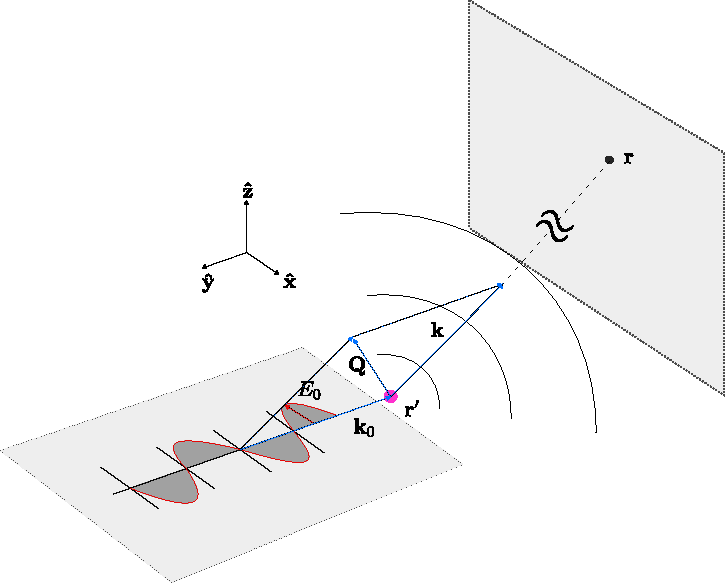
\includegraphics[width=\textwidth]{figures/Intro/scattering.pdf}
    \caption{Sketch of the scattering process evaluated in the far-field on the vertical plane for an electron density irradiated by a monochromatic X-ray beam 
    with linear polarization along the $\mathbf{\hat{x}}$ direction.}
    \label{fig:scattering}
\end{figure}

It is clear now that the information regarding the physical system of interest is embedded in the integral term. 
In fact, this is often called \textit{``form factor''} - $F(\mathbf Q)$ - and it plays an important role in the interpretation of the 
scattering equations. 

\begin{equation}
     F(\mathbf Q) = 
    \int_{\mathbb{R}^3} \rho(\mathbf r') e^{i \mathbf{Q} \cdot \mathbf{r}'}  d^3 \mathbf r'
    \label{eq:formfactor}
\end{equation}

This last term represents the Fourier transform of the electron density, and it is the main result of this paragraph as it 
links the charge distribution of the sample in real space with the quantity measured, in reciprocal space. 

To continue, we should bear in mind that X-ray photon counting detectors are sensitive to the time-averaged intensity 
of the signal as their time response is much slower than the oscillating frequency of X-rays ($\sim 10^{9}$ Hz for typical 
read-out limited frame rates of the Maxipix 
\cite{ponchut_maxipix_2011} against the $\sim 10^{18}$ Hz for X-rays at 10 keV). This limitation is also at the core of 
the ``Phase Problem'' that we will see later on, for which the phase information of the complex-valued wave-field is 
lost in the measurement. 
In order to do so, the time-averaged Poynting vector is calculated. 

\begin{equation}
    \langle \mathbf{S(r)} \rangle = r_e^2 \frac{1}{r^2}J_0
    \left| \int \rho(\mathbf{r'}) e^{i \mathbf{Q}\cdot \mathbf{r'}} d^3 r' \right|^2 \mathbf{\hat{r}}
    \label{eq:poynting}
\end{equation}

where $J_0 = \left| \mathbf{E}_0 \right|^2 / 2\mu_0c$ is the incident intensity. 
To conclude we consider the power delivered on the detector. For a pixel with area $d\mathbf a = r^2d\Omega\mathbf{\hat{r}}$ 
the radiation power is equal to: 

\begin{equation}
    P(\mathbf{Q})= r_e^2 J_0
    \left| \int \rho(\mathbf{r'}) e^{i \mathbf{Q}\cdot \mathbf{r'}} d^3 r' \right|^2 d\Omega
    \label{eq:power}
\end{equation}

Eq.\ref{eq:power} shows that the signal captured by the detectors is now in $\mathbf{Q}$ space, and it is proportional 
to the square modulus of the Fourier transform of the electron density of the sample. The square modulus operation also 
shows how the phase of the Fourier transformed scattering amplitude is lost.

\subsection{One atom}

If now we were to consider an atom, far from resonance, we could assume the electron density being the main responsible 
for the scattering. It is known indeed that protons, because of the larger mass, have a much smaller cross-section for the
scattering with photons. 
Using Eq.\ref{eq:formfactor} we would therefore have the \textit{atomic form factor} - $f_l(\mathbf{Q})$ being defined as: 

\begin{equation}
    f_l(\mathbf{Q} = 
   \int_{\mathbb{R}^3} \rho_l(\mathbf r) e^{i \mathbf{Q} \cdot \mathbf{r}}  d^3 \mathbf r
   \label{eq:atomformfactor}
\end{equation} 

We now need to study the specific case in which the collection of atoms is ordered into a periodic structure. 

\subsection{Ensemble of ordered atoms: a Crystal}

Perfect crystals are constructed by a basic structural arrangement of atoms (\textit{motif}) repeated periodically on a 
\textit{lattice} of one or more dimensions. The regularity of the lattice is such that, for the 3D case, any of its nodes 
can be located in space by the formula: 

\begin{equation}
   \mathbf {R_n} = n_1\mathbf{a_1} + n_2\mathbf{a_2} + n_3\mathbf{a_3}
   \label{eq:lattice}
\end{equation}

where ${\mathbf{a_1},\mathbf{a_2},\mathbf{a_3}}$ constitutes the basis vectors of the primitive unit cell and $n_1, n_2, n_3$ are integer numbers. 
It follows that the information can be condensed in the unit cell, i.e. the orientation in space of the basis vectors as any region 
of the lattice can be seen as the same unit cell, translated from the origin by the amount given by the $\sqrt{n_1^2 + n_2^2 + n_3^2}$. \\

The overall crystal is then constructed positioning on each of the nodes of the lattice the same motif, or basis. 

In another more elegant way, we could say that, being the lattice $\mathcal{L}(\mathbf r)$, the basis $\mathcal{B}(\mathbf r)$, the crystal 
$\mathcal{C}(\mathbf r)$ is given by the convolution of $\mathcal{L}(\mathbf r)$ with $\mathcal{B}(\mathbf r)$ : 

\begin{equation}
    \mathcal{C}(\mathbf r)  = \mathcal{L}(\mathbf r) \ast  \mathcal{B}(\mathbf r)
    \label{eq:conv}
 \end{equation}

 For simplicity, we will consider from now on a single atom basis.
 At this point, when evaluating the scattering amplitude of the crystal we have to deal to an assembly of atoms, and we 
 may want to exploit the regular structure we have just described. 
 First, we can assume that, similarly to the case of many scattering electrons, in the kinematical approximation the overall 
 scattering factor is given by the sum of the contributions of each atom, weighted by a phase factor that accounts for their 
 positions in space. 

 \begin{equation}
    F_{crystal}(\mathbf{Q}) = 
   \sum_{l=1}^{\text{All atoms}} f_l(\mathbf Q) e^{i \mathbf{Q} \cdot \mathbf{r_l}} 
   \label{eq:crystalformfactor}
\end{equation} 

Secondly, observing that the position of each atom is given by the sum of the position of the atom inside the unit cell 
and the lattice vector $\mathbf{r_l} = \mathbf{R_n} + \mathbf{r_j}$, we can separate Eq.\ref{eq:crystalformfactor} in two terms: 

\begin{equation}
    F_{crystal}(\mathbf{Q}) = 
   \sum_{\mathbf{R_n} + \mathbf{r_j}}^{\text{All atoms}} f_l(\mathbf Q) e^{i \mathbf{Q} \cdot (\mathbf{R_n} + \mathbf{r_j})} = 
    \underbrace{\sum_{n} e^{i \mathbf{Q} \cdot \mathbf{R}_n}}_{\text{Lattice}}
    \underbrace{\sum_{j} f_j(\mathbf{Q}) e^{i \mathbf{Q} \cdot \mathbf{r}_j}}_{\text{Unit cell}}
   \label{eq:crystalformfactor2}
\end{equation} 

The first summation extends over all lattice points, while the second covers all atoms within the unit cell. At this 
stage, we can once again take advantage of the lattice periodicity to evaluate the large summation over all lattice 
points. 

\subsection{Laue condition and Bragg's Law} 

The term we want to calculate is the sum of complex exponential, meaning that if the phases $\mathbf{Q} \cdot \mathbf{R_n}$ 
are misaligned the sum will be \textit{incoherent} and the resultant will be very small, in the order of unity. 
On the contrary, when phase offsets are equal to an integer multiple of $2\pi$ the \textit{phasors} will add \textit{coherently} 
The problem is thus to find those $\mathbf{Q}$ values for which

\begin{equation}
   \mathbf{Q} \cdot \mathbf{R_n} = 2\pi \times \text{integer}
   \label{eq:laue}
\end{equation}

In order to do than we need to construct a reciprocal space lattice with a set of basis ${\mathbf{a_1^\ast}, \mathbf{a_2^\ast}, \mathbf{a_3^\ast}}$ 
which fulfill: 

\begin{equation}
    \mathbf{a_1} \cdot \mathbf{a_1^\ast} = 2\pi h \qquad \mathbf{a_2} \cdot \mathbf{a_2^\ast} = 2\pi k \qquad \mathbf{a_3} \cdot \mathbf{a_3^\ast} = 2\pi l 
   \label{eq:miller}
\end{equation}

where $ h, k, l $ known as Miller indices, are integer. Having a set of basis vectors and the Miller indices, the 
resulting reciprocal space lattice lies in those points found by the vector $\mathbf{G}$ 

\begin{equation}
    \mathbf{G} =  h\mathbf{a_1^\ast} + k\mathbf{a_2^\ast} + l\mathbf{a_3^\ast} 
   \label{eq:G}
\end{equation}

This result is telling us that the scattering amplitude of a diffracting crystal is detectable only in those points in 
space for which the wave-vector $\mathbf{Q}$ coincides with a point of the reciprocal lattice, hence $\mathbf{Q} = \mathbf{G}$. 

This is known as the Laue condition for diffraction as it was discovered by Max von Laue in 1912 \cite{FriedrichKnippingLaue1912}.\\ 
A different but equivalent interpretation of the diffraction of a crystal was given by William Lawrence Bragg in 1913 \cite{Bragg1913}. 
Here, the crystal lattice is seen as a stack of parallel planes and the condition for constructive interference of 
the waves scattered by planes of the same family is found as follows.
Let us consider an X-ray beam of wavelength $\lambda$ and propagation vector $\mathbf{k_i} $ impinging with an angle $\theta$ 
on a crystal. We call $d$ the distance between the planes of the crystal. The scattered beam is leaving the crystal with the 
same angle $\theta$ and with a propagation vector $\mathbf{k_f}$ equal in magnitude to the incident one (\textit{elastic scattering}). 
At this point one can find the relationship between $ \theta, d, \lambda$ that allows for a constructive interference of the 
waves diffracted from the series of planes by evaluating the optical path length difference induced by the spacing. 
Reminding that $\left|k_i\right| = \left|k_f\right| = 2\pi/\lambda $ and with the help of Fig. \ref{fig:bragg} we can observe that this 
difference is $\Delta l = 2 d \sin(\theta)$ and therefore the phase offset between two waves is $\Delta \phi = \left|k\right| \Delta l 
= 4 d\pi \sin(\theta)/\lambda $. We have seen above that the condition for constructive interference requires the phase 
differences to be equal to a multiple of $2\pi$, therefore: 

\begin{equation}
    2 d \sin(\theta) = n \lambda 
   \label{eq:Bragg}
\end{equation}


Equation \ref{eq:Bragg} is known as Bragg's law, and it can be demonstrated to be equivalent the Laue condition, in scalar form. 
In particular, as illustrated in Fig.\ref{fig:bragg}, the scattering vector $\mathbf Q$ is equivalent to the vector G

\begin{figure}[H]
    \centering
    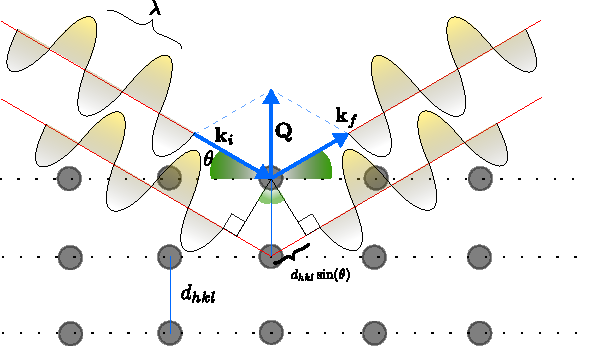
\includegraphics[width=\textwidth]{figures/Intro/bragg.pdf}
    \caption{Illustration of Bragg's law.}
    \label{fig:bragg}
\end{figure}


\subsection{Finite size crystals}

\subsection{Strained crystals}

\section{BCDI at ESRF - ID01}\label{chp:id01}

\subsection{Synchrotron radiation}

\subsection{Coherence}

\subsection{Ewald sphere and Rocking curves}

\subsection{Detectors}